\documentclass[conference]{IEEEtran}

\usepackage{xspace}
\usepackage{graphicx}
% \DeclareGraphicsExtensions{.pdf,.jpeg,.png}
% \usepackage{url}
%\usepackage[procnames]{listings}
\usepackage{paralist}
\usepackage{listings}
\usepackage{xcolor}
\usepackage{pbox}
\usepackage{subfig}

% No space between bibliography items:
\let\oldthebibliography=\thebibliography
  \let\endoldthebibliography=\endthebibliography
  \renewenvironment{thebibliography}[1]{%
    \begin{oldthebibliography}{#1}%
      \setlength{\parskip}{0ex}%
      \setlength{\itemsep}{0ex}%
  }%
  {%
    \end{oldthebibliography}%
  }

\renewcommand{\ttdefault}{pcr} % to fix non-bold key-words in listings
\lstdefinelanguage{conesc}
{
 morekeywords={components, triggers, is, error, default, context, group, layered, command, implementation, contexts, event, call, void, uses, transitions, iff, activate, interface},
 morecomment=[s]{/*}{*/},
 sensitive=false,
 escapeinside={*}{*}
 \setcounter{lstNoteCounter}{0}
}

\lstset{
  basicstyle=\scriptsize\ttfamily,
  keywordstyle=\bfseries,
  showstringspaces=false,
  emphstyle=\bfseries,
}

\definecolor{Lemon}{HTML}{FFFACD}
\lstdefinestyle{conescframe}{
  language=conesc,
  frame=lines,%single,
  xleftmargin=4mm,
  framexleftmargin=4mm,
  numbers=left,
  numberstyle=\scriptsize,
  numbersep=4pt,
  backgroundcolor=\color{Lemon}
}

% -begin- //nice in-code glyphs routine
\usepackage{tikz}
% for the pretty dark-circle-enclosed numbers
\newcommand*\circled[2]{\tikz[baseline=(char.base)]{
            \node[shape=circle,fill,inner sep=0.1pt, text=white,font=#2] (char) {#1};}}

\newcounter{lstNoteCounter}
\newcommand{\lstref}[1]{\circled{\ref{#1}}{\normalsize}}
\newcommand{\lstnote}[1] {
  \label{#1}\hbox to -8.5pt{\llap{{\circled{\ref{#1}}{\scriptsize\rmfamily}}\hskip 0.98em}}
}
% -end- //nice in-code glyphs routine

% correct bad hyphenation here
\newcommand{\lm}[1]{\footnote{{\bf Luca: #1}}}
\newcommand{\ma}[1]{\footnote{{\bf Mikhail: #1}}}

\newcommand{\conesc}{{\textsc{ConesC}}\xspace}
\newcommand{\code}[1]{{\bfseries\texttt{#1}}}

\newcommand{\fakepar}[1]{\vspace{0.4mm}\noindent\textbf{#1.}}
\newcommand{\wrt}{w.r.t.\ }

%\linespread{0.97}

\begin{document}

\title{Towards Self-adaptive Software\\for Resource-constrained Cyberphysical Systems}

% Author names and affiliations
% use a multiple column layout for up to two different
% affiliations


\author{\IEEEauthorblockN{Mikhail Afanasov}
\IEEEauthorblockA{Politecnico di Milano, Italy\\
afanasov@elet.polimi.it}
}

% \author{ 
% \alignauthor 
% %
% M.~Afanasov$*$, L. Mottola$*\dagger$ and C.~Ghezzi$*$\\
% %
% \affaddr{$*$Politecnico di Milano (Italy), $\dagger$SICS Swedish ICT} \\
% }

% make the title area
\maketitle

\begin{abstract}
  We present a context-oriented approach to develop self-adaptive
  software for extremely resource-constrained cyber-physical systems
  (CPSs). % These are sensing and actuating systems deployed in the
  % physical world whose operation is controlled by a computing and
  % communication core.
  Because of unpredictable environment dynamics, CPS software must be
  designed and implemented to dynamically adapt to widely different
  situations. Our approach provides design concepts and language
  support to achieve this against extreme resource constraints. To
  this end, we bring a notion of context-oriented design and
  programming down to platforms with only a few KBytes of memory and
  currently leveraging rather basic programming environments. Early
  results demonstrate that our approach greatly simplifies the design
  and implementation of adaptive CPS software at the price of a modest
  system overhead. To our knowledge, we are the first to enable
  context-oriented design and programming in similarly-constrained
  platforms.
\end{abstract}


%%% Local Variables: 
%%% mode: latex
%%% TeX-master: "paper"
%%% End: 

\section{Introduction}

Cyberphysical systems (CPSs) gather data from and take actions on the real
world. The environmental dynamics determines the requirement for CPS software to
be adaptable. Moreover, adaptation should occur simultaneously along diferent
dimensions. In wildlife tracking applications~\cite{pasztor10:selective}, for
example, sensor nodes are attached to animals to study their movements, social
interactions, and health conditions. Nodes are running on batteries, which makes
the energy a precious resource. To save it, such devices as GPS and radio should
be disabled when not needed. Orthogonally, the node should send the data to the
base-station, if it is reachable, or save it locally otherwise.

In the absence of design-time support for self-adaptive software, the adaptation
described above would be achieved by ad-hoc
code~\cite{Zimmerling12,Bourdenas11}, that makes the application cumbersome to
design, and difficult to understand, debug, and maintain. A more general
approach -- context-oriented programming (COP)~\cite{Hirschfeld08} -- addresses
these issues by providing a design-time abstractions for adaptations. There are
many implementations of COP in high-level
languages~\cite{Ghezzi10,Salvaneschi12,Sehic11}, most of which are not
applicable to embedded systems, because of resource limitations.

%Many works exist in the area of self-adaptive embedded
%systems~\cite{Zimmerling12,Bourdenas11}, which illustrates a problem-specific
%approach dedicated code. A more general approach -- context-oriented
%programming (COP)~\cite{Hirschfeld08} -- is implemented in several high-level
%languages~\cite{Ghezzi10,Salvaneschi12,Sehic11}. Most of them are not
%applicable to the embedded systems, because of resource limitations.

By borrowing COP concepts and bringing them down to low-level CPS software, we
provide a design-time and programming support to enable self-adaptive behavior.
As a result, we introduce \conesc -- a context-oriented extension of nesC
language -- in Sec.~\ref{sec:concepts}, where we also describe the concepts the
language was build upon. We discuss our preliminary evaluations in
Sec.~\ref{sec:eval}, and open problems in Sec.~\ref{sec:future}.

\section{Design Concepts}\label{sec:appdesign}

We illustrate in the following language-independent design concepts,
providing a foundation to apply the COP model to different concrete
languages, as we further illustrate next. Throguhout this section and
the next, we refer to the wildelife tracking application described
earlier as a running example.

We define two key concepts:~\emph{i)} individual contexts, and
\emph{ii)} context groups. Contexts represent the different
environmental situations the system may encounter, and correspond to
behavioral variations associated to a given situation. As the
environment surrounding the system mutates, the software adapts
accordingly by activating given contexts. Context groups represent
collections of contexts sharing common characteristics; for example,
whenever the same functionality must adapt to changes in the
surrounding environment or the required adaptive behavior is
determined by the same environmental quantity. We argue that these
concepts are sufficient to capture a wide range of adaptive behaviors
in WSNs, and yet are largely independent of a specific programming
language.

% Programming in \conesc is intimately tied with environment-dependent behavior of
% the application and exploits two main concepts: \emph{i)} individual contexts
% and their transitions and \emph{ii)} context groups. The former represent
% different environment situations where a system may find itself. Each context
% maps to a separate state of the device or environment a system operates in. As
% the environment conditions change, a programmer initiates a context transition
% by \emph{activating} the corresponding context. A context group is a set of
% contexts sharing common characteristics and variations of the same
% functionality. Thus, whenever a transition between involved contexts occurs, it
% is determined by changes in one or more physical quantities.

\putfigure{caption=Wildlife tracking diagram.,label=fig:wtd}{
 \centering
 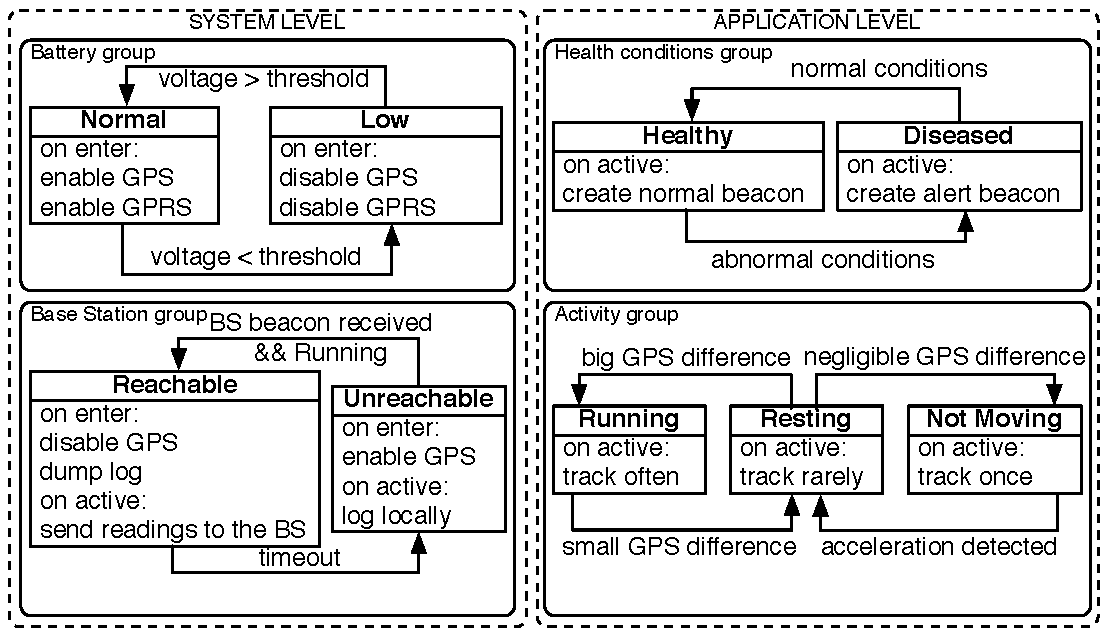
\includegraphics[width=\columnwidth]{pdf/wildlifetracking}
}

Fig.~\ref{fig:wtd} exemplifies how programmers use these concepts in
the design of the wildlife tracking application. Context groups are
defined to describe behavioral variations corresponding to different
battery levels and whether a node is within the communication range of
a base-station, as well as an animal's health conditions and
activity. Context groups are tagged as system-level or
application-level to discern application-specific functionality from
likely re-usable system services.

The contexts within a group define the individual behavioral
variations depending on the situation. For example, the function to
report sensor readings and contact traces must behave differently
depending on whether the base-station is reachable.  If so, the data
may be relayed immediately to the base-station using the radio. To
this end, the programmer activates context \emph{Reachable} within the
\emph{Base-station} group. Otherwise, the programmer activates context
\emph{Unreachable}, as the software must log the data locally; for
example, on flash. 

The contexts in a group are tied with transitions that
express the conditions triggering the context change. For example,
within the \emph{Base-station} group, the system transitions from
context \emph{Reachable} to \emph{Unreachable} whenever no beacons are
received from the base-station within a timeout. This entails
a node is out of the base-station communication range and the software
must adapt accordingly, that is, by locally storing the contact logs
instead of sending them over the radio.

% Orthogonal to application-level functionality, the system should transmit data
% to the Base Station (BS) or save readings locally depending on the BS
% availability. Whenever the latter is \emph{Unreachable}, a node logs data in
% internal memory, but should it receive a BS-beacon, the data is dumped to the
% BS. Crucially, the node runs on a battery, so the system should be aware of a
% battery status and disable GPS-module, which is power consuming, if the battery
% level is \emph{Low}.

The behavioral variations must not necessarily implement a complete
functionality on their own, but they may also serve other
functionality; for example, by providing context-dependent data. The
group \emph{Health conditions} is one such example. By using a body
temperature sensor, the system detects whether the animal is
\emph{Diseased} or \emph{Healthy}. The corresponding behavioral
variations implement two ways to build the radio beacon used as a
proximity sensor for detecting contacts between animals. If the animal
is \emph{Diseased}, additional information is added to the beacon for
understanding how the disease spreads. Either type of beacon is then
handed over to the radio stack for transmission.

The concepts we outlined suffice to organize the environment-dependent
functionality in a large class of WSN applications, as we further
argue in Section~\ref{sec:eval}. On the other hand, unlike the vast
majority of WSN programming approaches~\cite{mottola11survey}, these
concepts remain largely decoupled from a concrete language
implementation. Although the following section describes a
nesC-based implementation---mainly motivated by the availability of a
mature toolchain---our design can be straightforwardly embedded within
other WSN languages. For example, within functional lanuages such as
Regiment~\cite{} or Flask~\cite{}, one would simply enable behavioral
variations of programmer-defined functions through a proper syntax,
together with dedicated keywords for context transitions.


% By using a body temperature sensor
% system detects if an animal is \emph{Diseased} and builds an alert
% beacon or a normal beacon otherwise. Here contexts \emph{Healthy} and
% \emph{Deseased} are based on a physical quantity -- the body
% temperature of an animal -- and reflect variations of the same
% functionality, such as building a beacon, so they can be joined into a
% group \emph{Health conditions}.


% Depending on GPS readings developers may want to vary a sampling rate to use
% energy more effective. For example, there is no need to track a location if an
% animal is \emph{NotMoving}, but should accelerometer detect any significant
% movement, a periodic sampling should be initiated. Increased difference between
% two location readings indicates that an animal is \emph{Running}, and location
% sampling should occurs more often.

% \conesc reflects this design by using new types of components, such as
% \emph{context} and \emph{context group} -- extensions of \emph{module} and
% \emph{configuration} correspondingly -- and a set of new key-words. Instances of
% new types, however, can also be used as standard nesC components, e.g. they can
% provide or use interfaces as well as be declared in the same way.

%%% Local Variables: 
%%% mode: latex
%%% TeX-master: "bare_conf"
%%% End: 

\section{Evaluation}\label{sec:eval}

For evaluation purposes, we implemented three applications. For each we compare
nesC implementation against its \conesc counterpart.

{\bf Complexity} is estimated by using such metrics as the number of lines of
code (LOC), the number of variables declared and functions
defined~\cite{Pressman01}. Despite our results show 30\% increase of average
complexity, there is significant reduction in average per-module complexity --
-54\%. We believe that in larger applications the number of the similar lines of
code will be bigger. Nevertheless, \conesc-written applicaton is more than 3
times smaller than generated code, what makes \conesc an effective tool for
context-oriented programming.

{\bf Overhead} in terms of memory is lesser than
2,5\% for binary size and less than 4,5\% for RAM overhead. The average CPU
overhead for layered function calls oscillates from 2 to 5 CPU cycles depending
on application, which is negligible in terms of energy consumption, since the
simplest operation in TinyOS -- turn on/off LEDs -- consumes 8 CPU cycles. The
context transitions overhead is bigger -- from 10 to 25 CPU cycles -- but
remains in the same order of magnitude.

\section{Future work}

An open problem of our research are possible conflicts and nontrivial
logical errors of context-oriented model of the application. To leverage it, we
put a domain-specific model checking in our research agenda.

To our knowledge there is also a lack of programming environment for
self-adaptive applications for CPSs. Our early analysis shows that complexity
can be decreased by 9\%, if the skeleton of the application based on the diagram
akin to the one in Figure~\ref{fig:design} is generated by IDE.

Another direction of our research is to investigate context-oriented programming
for other CPS platforms, such as aerial drones.

\section{Biography}

Mikhail Afanasov is a second year student of a 3-year PhD program at the
Department of Electronics and Information (DEI) of Politecnico di Milano. He was
accepted there in November 2012 after receiving Masters degree in "Applied
Physics and Mathematics" at Moscow Institute of Physics and Technology (2012).

He has a pleasure to conduct his research in tight collaboration with Carlo
Ghezzi and Luca Mottola in the area of designing self-adaptive software for
extremely resource-constrained cyber-physical systems

% acknowledgements
{\small
\bibliographystyle{abbrv}      % 
\bibliography{bibl}   % name your BibTeX data base
}

% ACM needs 'a single self-contained file'!
%
%APPENDICES are optional
%\balancecolumns
%\appendix
%Appendix A

\end{document}


